\subsubsection{Pooling Layer}
\label{sec:cnn-pooling-layer}
After obtaining features using a convolutional layer a pooling layer can be inserted working on their activations.
Pooling serves as a spatial dimension reduction.
This is done by moving a filter $\vec{K} \in \mathbb{R}^{i \times j}$ with a given stride $s$ over an input $\vec{I} \in \mathbb{R}^{u \times v}$ that compresses the information or values, respectively, within its window.
However, the depth is usually not compressed and stays the same.
The objective of this process is to remove unnecessary information while keeping important features and improving computational power as less spatial information is available.
Hence, fewer weights and biases are needed which in turn improves training time.
\figref{fig:pooling} illustrates the pooling process for a max pooling operation in practical terms.
A max pooling filter $\vec{K}_{\text{max}}$ yields the maximum within its window as the result.
Moving such a $2 \times 2$ filter over an $4 \times 4$ input $\vec{I}$ with a stride of $s=2$ yields a matrix with each maximum at its corresponding position.
The maximum of the red colored $2 \times 2$ window is 7, hence, this number comes up in the result.
The other windows are processed identically.
The size of the result of an arbitrary pooling operation can be calculated with \eqref{eq:feature-map-shape} and $\dim \left( \vec{F} \right)_3 = \dim \left( \vec{I} \right)_3$.
Another pooling type is mean pooling.
Hereby, the result of each window is the mean of all its values.
In many architectures max pooling outperforms mean pooling \cite{Scherer2010}, however, in general, the type of pooling is problem-specific.
As it can be seen, pooling layers do not have learnable parameters only hyperparameters.
\begin{figure}
	\centering
	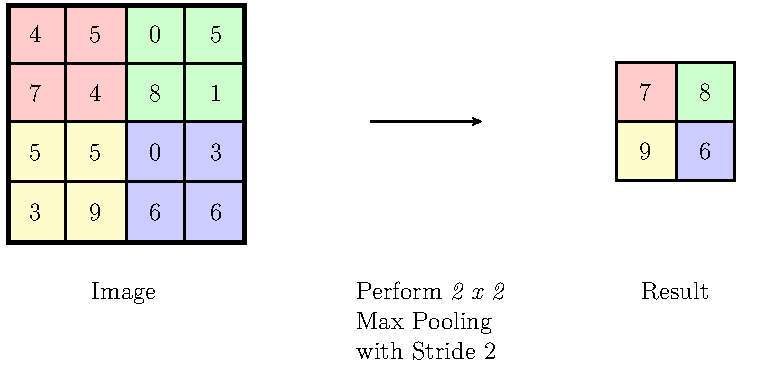
\includegraphics{images/pooling.pdf}
	\caption[Max pooling with $2 \times 2$ filter and stride $2$]{Max pooling with $2 \times 2$ filter $\vec{K}_{\text{max}}$ across a $4 \times 4$ input $\vec{I}$ with a stride of $s=2$. Within each window, the maximum of its values is computed. Finally, this yields a matrix with each maximum at its corresponding position.}
	\label{fig:pooling}
\end{figure}